%\tikzstyle{decision} = [
  diamond,
  very thick,
  draw=red!50!black!50,
  %fill=red!20, 
  aspect=2,
  %text badly centered,
  top color=white,
  bottom color=red!50!black!20,
]
\tikzstyle{stmt} = [
  rectangle,
  very thick,
  draw=blue!50!black!50,
  %fill=blue!20, 
  text centered,
  minimum height=5ex,
  minimum width=5em,
  top color=white,
  bottom color=blue!50!black!20,
]
\tikzstyle{node} = [
  circle,
  very thick,
  draw=orange!50!black!50,
  fill=orange!20,
  minimum size=6ex,
]
\tikzstyle{io} = [
  very thick,
  draw=green!50!black!50,
  trapezium,
  trapezium left angle=80,
  trapezium right angle=-80,
  %fill=green!20!black!10,
  %rounded corners,
  %minimum height=5ex,
  top color=white,
  bottom color=green!50!black!20,
  text centered,
  minimum height=5ex,
  minimum width=5em,
]
\tikzstyle{conn} = [very thick, draw=black!50, -latex']


\tikzstyle{place}=[circle, draw, fill=black, inner sep=0pt, thick, minimum size=2mm]
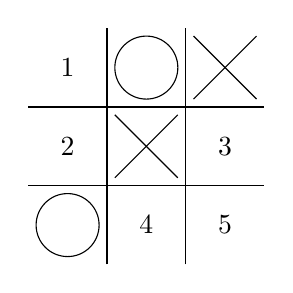
\begin{tikzpicture}
	\draw (1,0) -- (1,3);
	\draw (2,0) -- (2,3);
	\draw (0,1) -- (3,1);
	\draw (0,2) -- (3,2);

	\draw (0.5,2.5) node {1};
	\draw (0.5,1.5) node {2};
	\draw (0.5,0.5) circle (.4);

	\draw (1.5,2.5) circle (.4);
	\draw (1.1,1.1) -- +(.8,  .8);
	\draw (1.1,1.9) -- +(.8, -.8);
	\draw (1.5,0.5) node {4};

	\draw (2.1,2.1) -- +(.8,  .8);
	\draw (2.1,2.9) -- +(.8, -.8);
	\draw (2.5,1.5) node {3};
	\draw (2.5,0.5) node {5};

\end{tikzpicture}
